\documentclass{article}
\usepackage[utf8]{inputenc}
\usepackage{amsmath, amsfonts, amssymb}
\usepackage[margin = 1in]{geometry}
\usepackage{listings}
\usepackage{fancyhdr}
\usepackage{graphicx}
\usepackage{listings}
\usepackage{url}

% Allows us to use subfigures
\usepackage{caption}
\usepackage{subcaption}

\lstset{
	literate={~} {$\sim$}{1},
	belowcaptionskip=1\baselineskip,
	breaklines=true,
	frame=L,
	xleftmargin=\parindent,
	language=R,
	showstringspaces=false,
	basicstyle=\ttfamily
}

\pagestyle{fancy}
\fancyhead[L]{Variable Selection Techniques}
\fancyhead[R]{G. Ackall, C. Shrader}
\fancyfoot{}
\fancyfoot[C]{\thepage}

\setlength{\parskip}{6pt}

\title{Variable Selection Techniques}
\author{Gabriel Ackall and Connor Shrader}
\date{\today}

\newcommand{\argmin}[1]{\underset{\beta}{\text{arg min}}}
\newcommand{\sign}{\text{sign}}

\begin{document}
\maketitle

\section{Introduction}
Linear regression is one of the simplest forms of statistical learning models. It assumes that some predictor variable $y$ can be modeled as a linear combination of a set of predictor variables $x_1, x_2, \dotsc, x_p$. More precisely, a linear regression model assumes that
\begin{equation}\label{eqn:linear-model}
	y = \beta_0 + \beta_1 x_1 + \beta_2 x_2 + \cdots + \beta_p x_p + \epsilon
\end{equation}
where $\beta_0, \beta_1, \dotsc, \beta_p$ are coefficients and $\epsilon$ is a random error with mean zero and variance $\sigma^2$. We also assume that this error has no correlation between different observations. When working with real data sets, the coefficient values are usually unknown; the goal of linear regression is to compute coefficient estimates $\hat{\beta_0}, \hat{\beta_1}, \dotsc, \hat{\beta_p}$ that are good estimates for the actual coefficients.

\subsection{Ordinary Least Squares}

Let $\beta = [\beta_0, \beta_1, \dotsc, \beta_p]^{T}$ be a vector of coefficient values, and let $\hat{\beta} = [\hat{\beta}_0, \hat{\beta}_1, \dotsc, \hat{\beta}_p]^{T}$ represent a vector of coefficient estimates. Let $\mathbf{X}$ be a $n\times(p + 1)$ matrix containing $n$ observations in $p$ variables. In order to account for the constant $\beta_0$ term in Equation \ref{eqn:linear-model}, we include an extra column in $\mathbf{X}$ with each entry equal to 1; the coefficient estimate for this additional ``variable'' will be $\hat{\beta}_0$. Finally, let $\mathbf{y}$ represent the vector of response values for each observation.

The most common way to compute $\hat{\beta}$ is with ordinary least squares. This method computes $\hat{\beta}$ by minimizing the residual sum of squares:
\begin{align}
	\hat{\beta}^{\text{OLS}} &= \argmin{\beta}\left\{\sum_{i=1}^{n} \left( y_i - \beta_0 - \sum_{j=1}^{p} \beta_jx_{ij} \right)^2 \right\}\\
	&= \argmin{\beta} \left\{ (\mathbf{y} - \mathbf{X}\beta)^\top (\mathbf{y} - \mathbf{X}\beta)^\top\right\}
\end{align}
Ordinary least squares is favored for a few reasons. For one, the solution is very easy to compute; the coefficient estimate is given by
\begin{equation}
	\hat{\beta} = (\mathbf{X}^\top\mathbf{X})^{-1}\mathbf{X}^\top\mathbf{y}
\end{equation}
Another advantage of ordinary least squares comes from the Gauss-Markov Theorem. This theorem states that of all the linear unbiased estimators, ordinary least squares has the lowest variance. Alternative unbiased estimators will necessarily have a larger variance, which can lead to more inaccurate predictions.

\subsection{Linear Regression with High Dimensionality Data}

If ordinary least squares minimizes variance among all unbiased estimators, why would we use anything else? One issue is that the matrix $\mathbf{X}^\top\mathbf{X}$ is not always invertible. In fact, this matrix is never invertible in the case when $p>n$. Hence, in some situations, we cannot use ordinary least squares.

Even if the matrix is invertible, other methods may lead to better model performance. Despite having the least variance among unbiased estimators, ordinary least squares may still have high variance. Consequently, it may be worthwhile to sacrifice some bias in order to reduce variance.

Many biased linear regression models perform \textit{variable selection}, meaning that some coefficient estimates will be set to zero. In many applications, not all of the predictors will be related to the response, but ordinary least squares still attempts to use every predictor when computing coefficient estimates. Variable selection techniques can identify the predictors most strongly correlated to the data and eliminate the rest. This results in a simpler model that uses $p^\ast$ of the $p$ available predictors. This not only helps reduce variance, but it also creates more interpretable models.

The rest of this document examines many approaches to fitting linear regression models. These techniques fall under two categories: subset selection and penalized regression. Subset selection algorithms attempt to find a subset of predictors that is most strongly correlated to the response and  fits an ordinary least squares model to that subset. Penalized regression techniques punish large coefficient estimates, which encourages models that have smaller coefficient values. Depending on the particular algorithm used, penalized regression can also perform variable selection.

\subsection{Alternative Techniques with High Dimensionality Data}
In addition to penalized and subset selection linear regression methods used for variable selection, there are other techniques that can achieve similar results. One of these such methods includes using boosting. Boosting achieves accurate predictions by sequentially updating inaccurate models, each time correcting on the weaknesses of the predecessor. While boosting is traditionally used with decision trees and classification, its premise has shown success with linear models and regression, as demonstrated by Buehlmann et. al. \cite{buehlmann2006boosting}.

Random forest techniques have also shown promise and perform very well for high dimensionality data. However, they are limited in that they do not perform as well when the number of predictors is greater than the number of data samples. This is because random forests work by using the majority vote of thousands of decision trees on bootstrapped data. Due to the lack of samples, tree pruning can lead to increased error, and this can contribute to overfitting where the model fits the training data well, but cannot capture the true relationships of the data. This will lead to decreased accuracy when exposed to new testing data \cite{genuer2008random}. Still, random forest is a common model used when the number of predictors is greater than the number of samples and recently, some statisticians have proposed new random forest methods that perform much better than traditional methods \cite{capitaine2021random}.

\section{Subset Selection}
First, we discuss subset selection techniques. In general, these techniques are discrete algorithms that attempt to find a good model using only a subset of the available predictors.
\subsection{Best Subset Selection}
Best subset selection is a method for selecting the most influential predictors that minimize error in a least squares linear regression. It does this by fitting a linear regression model to every possible combination of predictors and then choosing the best model of all the possible combinations. The best model is determined through the use of a test error estimate. The most common examples of test error estimation indicators are Akaike information criterion (AIC), Bayesian information criterion (BIC), Adjusted $R^2$, and cross validation.

While best subset selection results in the best possible model given the predictors, it is very computationally expensive. As the number of predictors increases, the number of linear models that best subset selection has to fit increases exponentially. This can be seen in Table \ref{tab:subset-combinations}. Thus, for models with more than 40 predictors, this can become infeasible for most computers to compute \cite{james2013introduction}. Given that in many scenarios, especially those seen in medicine with genomic data or in scenarios where there are more predictors than data samples, there can be many thousands of predictors, and best subset selection becomes impossible.

\begin{table}[h!]
	\centering
	\caption{Number of fitted models depending on number of predictors (p)}
	\vspace{0.1in}
	\begin{tabular}{c|r@{\hskip 4pt}l}
		\hline
		p  &  \multicolumn{2}{c}{Fitted Models}\\
		\hline
		2   & $2^2$ & $=4$ \\
		10  & $2^{10}$ & $=1024$ \\
		100 & $2^{100}$ & $>10^{30}$ \\
		k   & $2^k$ & \\
	\end{tabular}
\label{tab:subset-combinations}
\end{table}

Figure \ref{fig:best-subset-selection} below demonstrates how the number of predictors can affect $R^2$ and BIC when using best subset selection. This plot was created by using the \lstinline!leaps! library (which provides a function to run best subset selection) \cite{lumley2020leaps}. We used the \lstinline!College! dataset provided by the \lstinline!ISLR! library \cite{james2017islr}, and fit linear regression models using \lstinline!Grad.Rate! as the response. We see that as the number of predictors increases, $R^2$ always increases (as expected). On the other hand, BIC is minimized with a moderate number of variables (between seven and nine). According to the BIC statistic, the best model has seven variables. The code used for this figure is in the \lstinline!r! folder of the REU GitHub repository.

\begin{figure}[!h]
	\centering
	\caption{$R^2$ and BIC when applying best subset selection}
	\label{fig:best-subset-selection}
	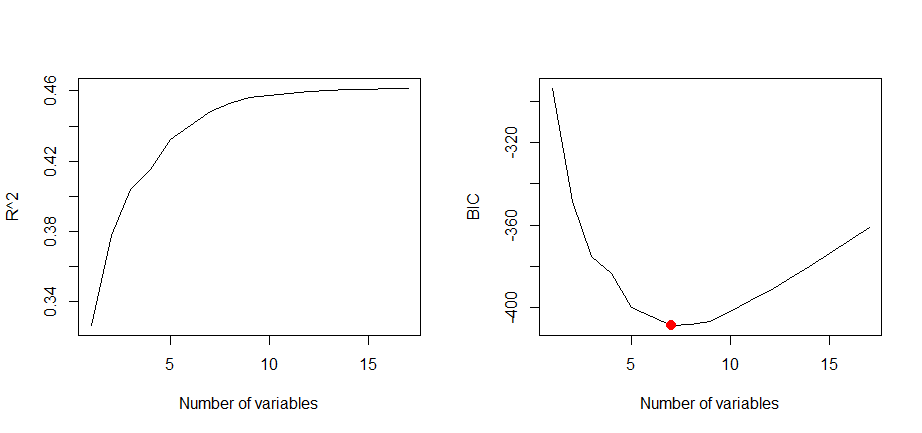
\includegraphics[width = 6in]{images/best-subset-selection.png}
\end{figure}

\subsection{Forward Stepwise Selection}
Forward stepwise selection aims to approximate the best combination of predictors in a linear regression model, but with a more computationally efficient method than best subset selection. Forward stepwise selection starts without using any predictors. It then slowly begins adding the most important predictor to the model. The predictor is chosen to minimize statistics such as p-value, AIC, BIC, or Adjusted $R^2$, to name a few. This is repeated until a stopping point is reached which can be defined by p-value, AIC, BIC, and more.

This process is much more computationally efficient than best subset selection, but it does not necessarily result in the best combination of parameters in the linear regression and is not guaranteed to result in the best model.

Figure \ref{fig:forward-stepwise-selection} shows the $R^2$ and BIC statistics when fitting models using forward stepwise selection. Again, we predicted \lstinline!Grad.Rate! using the \lstinline!College! data set using the \lstinline!leaps! library. The results are almost identical to what we saw for best subset selection. Even though the plots are similar, the specific model chosen by forward stepwise selection is actually different than the one found using best subset selection.

\begin{figure}[!h]
	\centering
	\caption{$R^2$ and BIC when applying forward stepwise selection}
	\label{fig:forward-stepwise-selection}
	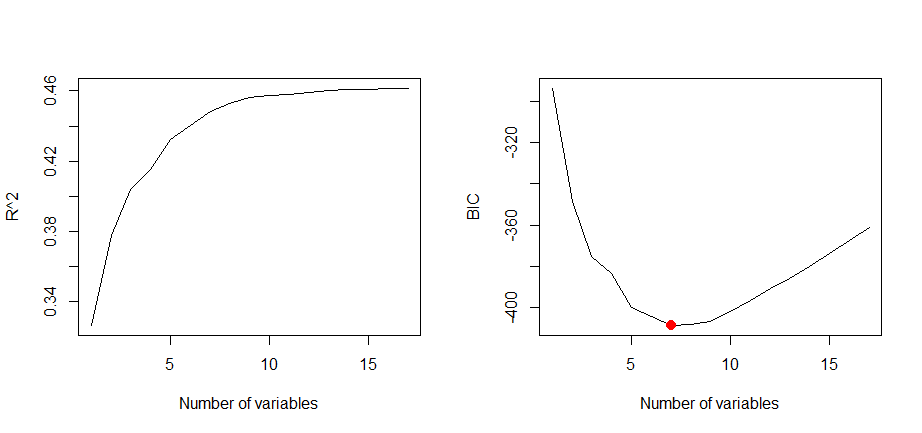
\includegraphics[width = 6in]{images/forward-stepwise-selection.png}
\end{figure}

\subsection{Backward Stepwise Selection}
Backwards stepwise selection works very similarly to forward stepwise selection, except that it starts with every single predictor included in the least squares linear regression. Instead of adding predictors like in forward stepwise selection, backward stepwise selection removes the least important predictor in each iteration. Similar to the forward method, the importance of a predictor can be determined by its p-value, AIC, BIC, or Adjusted $R^2$. This is repeated until a pre-determined stopping point is reached.

Backward stepwise selection can often result in better models than forward stepwise selection because it is guaranteed to test all the predictors together. This is different from forward stepwise selection that can sometimes suppress predictors, especially those that are collinear. For these reasons, when its use is possible, backward stepwise selection is preferred to forward stepwise selection. However, in cases where the number of predictors are greater than the number of samples, backward stepwise selection is impossible. In these case, forward stepwise selection must be used.

Figure \ref{fig:backward-stepwise-selection} shows $R^2$ and BIC after applying backward stepwise selection to the \lstinline!College! data set. Again, the results are very similar to Figures \ref{fig:best-subset-selection} and \ref{fig:forward-stepwise-selection}, but the particular models chosen by the algorithm were slightly different. 

\begin{figure}[!h]
	\centering
	\caption{$R^2$ and BIC when applying backward stepwise selection}
	\label{fig:backward-stepwise-selection}
	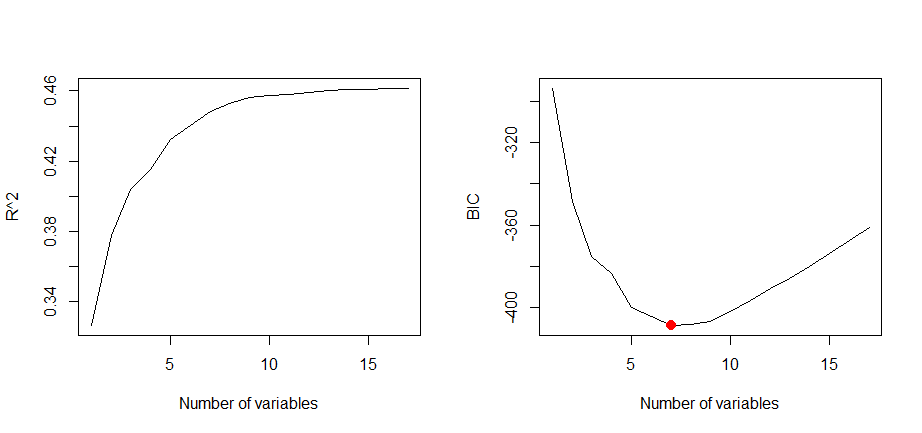
\includegraphics[width = 6in]{images/backward-stepwise-selection.png}
\end{figure}

\subsection{Hybrid Stepwise Selection}
One weakness of the forward stepwise and backward stepwise methods is that they are greedy algorithms; in general, they will not find the best model for a given number of predictors. One way to improve model accuracy is to use hybrid stepwise selection, which allows for both forward steps and backward steps \cite{friedman2001elements}.

The algorithm could start with either zero predictors or all predictors. In each iteration, the method would either add a new predictor to the model or remove a predictor that does not increase performance. Like the forward and backward stepwise selection methods, this algorithm terminates when the model cannot be improved further; measuring the accuracy of the model can be determined using the AIC or BIC.

Although this strategy is slightly more computationally expensive than forward stepwise or backward stepwise selection, a hybrid approach may improve model results while still avoiding the unrealistic runtime of best subset selection.

\subsection{Forward Stagewise Selection}
One last method for feature selection is called forward stagewise regression. Like forward stepwise selection, forward stagewise selection starts by fitting a model using none of the predictors. In each iteration, the method chooses the predictor most closely correlated to the residuals of the current model, and fits a simple linear regression using the predictor against the residuals. The coefficient for this predictor in the simple model is then added to the corresponding coefficient in the other model. This process is repeated until none of the predictors are correlated with the residuals.

Note that in each iteration of this algorithm, only one of the coefficients is changed. As a result, this method has a long runtime. In the long run, forward stagewise selection is still competitive compared to the strategies previously discussed.

\section{Penalized Regression}
The following sections discuss several modifications to the ordinary least squares model that penalize large coefficient estimates. Recall that an ordinary least squares model assumes that some response variable $y$ can be modeled by

\begin{equation}
	y = \beta_0 + \beta_1 x_1 + \beta_2 x_2 + \cdots + \beta_p x_p + \epsilon
\end{equation}

where $x_1, x_2, \dotsc, x_p$ are predictors, $\beta_0, \beta_1, \dotsc, \beta_p$ are coefficients, and $\epsilon$ is some random error with mean 0 and variance $\sigma^2$. An ordinary least squares model estimates the coefficients as

\begin{equation}
	\hat{\beta}^{\text{OLS}} = \argmin{\beta}\left\{\sum_{i=1}^{n} \left( y_i - \beta_0 - \sum_{j=1}^{p} \beta_jx_{ij} \right)^2 \right\}
\end{equation}

In general, a penalized regression imposes some additional restriction that punishes large coefficient estimates. The coefficient estimates are then given by
\begin{equation}
	\hat{\beta} = \argmin{\beta}\left\{ \sum_{i=1}^{n} \left( y_i - \beta_0 - \sum_{j=1}^{p} \beta_jx_{ij} \right)^2 + \sum\limits_{j = 1}^p p(\beta_j) \right\}
\end{equation}
where $p(\beta_j)$ is some penalty function. Generally, this function should be large when the coefficient is large so that a model with smaller coefficients is favored. Penalized regression is especially useful when $p>n$ because the penalties can reduce variance and perform variable selection at the cost of some bias.

Because these models place penalties on large coefficient estimates, it is common to standardize the predictors to have a mean of 0 and a variance of 1. This ensures that none of the predictors have a disproportionate effect on the estimated coefficients.

\subsection{Ridge Regression}
Ridge regression helps to solve multicollinearity in predictors while also minimizing insignificant predictors. While it does not minimize these insignificant predictors completely to 0 and thus cannot be considered a variable selection method, it still proves very useful in large datasets.

Ridge regression works by minimizing Residual Sum Squared (RSS) plus a penalty as seen in Equation \ref{ridge_reg}. $\lambda$ is a tuning parameter and can be used to determine how much of an effect the penalty has on the regression. if $\lambda=0$, then the regression acts exactly like ordinary least squares regression, but if $\lambda \rightarrow \infty$, then $\beta_j \rightarrow 0$ and the regression line will be a horizontal line at the intercept, $\beta_0$.

\begin{equation}
	\hat{\beta}^{\text{ridge}} = \argmin{\beta}\left\{ \sum_{i=1}^{n} \left( y_i - \beta_0 - \sum_{j=1}^{p} \beta_jx_{ij} \right)^2 + \lambda \sum_{j=1}^{p} \beta_j^2  \right\}
	\label{ridge_reg}
\end{equation}

An alternative way to express ridge regression is with the equation
\begin{equation}
	\hat{\beta}^{\text{ridge}} = \argmin{\beta}\left\{ \sum_{i=1}^{n} \left( y_i - \beta_0 - \sum_{j=1}^{p} \beta_jx_{ij} \right)^2\right\}\quad\text{subject to}\quad \sum_{j=1}^{p} \beta_j^2\leq t
\end{equation}
for some tuning parameter $t$.

\subsection{Lasso Regression}

The least absolute shrinkage and selection operation, often referred to as \textit{lasso}, is a shrinkage method with a very similar form to lasso regression \cite{tibshirani1996regression, james2017islr, james2013introduction}. The coefficient estimates satisfy
\begin{equation}
	\hat{\beta}^{\text{lasso}}=\argmin{\beta}\left\{ \sum\limits_{i = 1}^n \left( y_i - \beta_0 - \sum\limits_{i = 1}^p \beta_j x_{ij} \right) + \lambda\sum\limits_{j = 1}^p \vert \beta_j \vert \right\}
\end{equation}
If $\lambda = 0$, then the lasso model is equivalent to the ordinary least squares model; if $\lambda \to \infty$, then the coefficients for all predictors will be set to 0. An equivalently way to define lasso regression is by
\begin{equation}
	\hat{\beta}^{\text{ridge}} = \argmin{\beta}\left\{ \sum_{i=1}^{n} \left( y_i - \beta_0 - \sum_{j=1}^{p} \beta_jx_{ij} \right)^2 \right\}\quad\text{subject to}\quad \sum_{j=1}^{p} \vert \beta_j \vert\leq t
\end{equation}
where $t$ is a tuning parameter.

One useful property of the lasso method is that it can perform variable selection by setting some coefficients to zero. To understand why lasso regression can perform variable selection whereas ride regression cannot, consider Figure \ref{fig:ridge-lasso} below. This figure demonstrates the case when $p=2$ and $t = 1$. The red diamond on the left represents the condition $\vert \beta_1 \vert + \vert \beta_2 \vert < 1$ for ridge regression, while the circle on the right represents the condition $\beta_1^2 + \beta_2^2 < 1$ for lasso regression. The black curves represent contours of the residual sum of squares error for values of $\beta_1$ and $\beta_2$. The black point in the center of these curves is where the RSS is minimized; this represents the values of $\beta_1$ and $\beta_2$ that would be selected by ordinary least squares.

\begin{figure}[!h]
	\centering
	\caption{Error and constant curves for the lasso and ridge models when $p=2$.}
	\label{fig:ridge-lasso}
	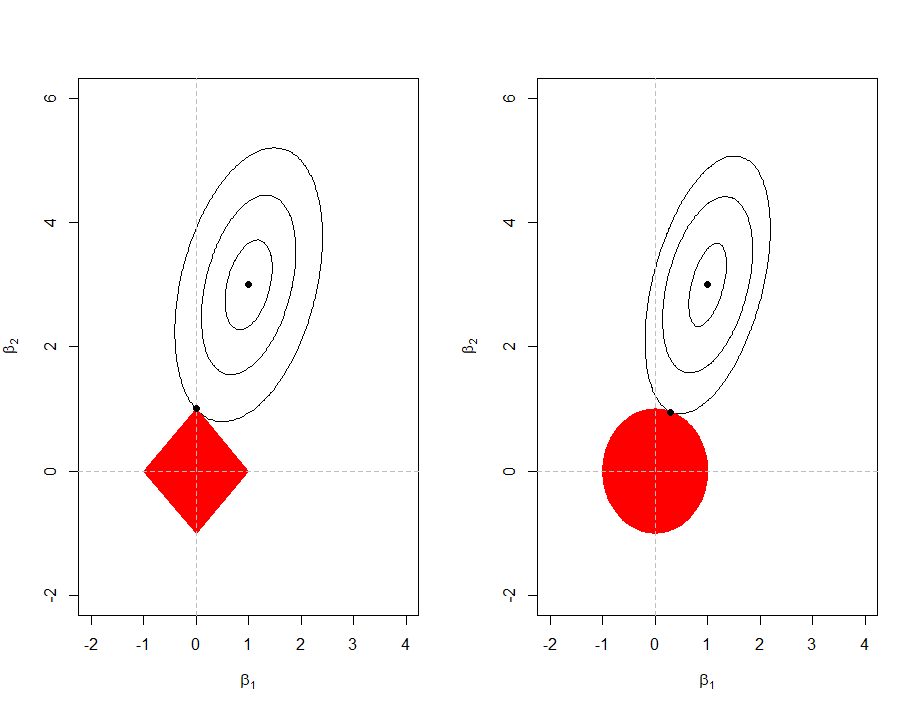
\includegraphics[width = 0.6\textwidth]{images/ridge-lasso.png}
\end{figure}

In the left plot, the intersection of the black curve and the red diamond represents the parameter values chosen by lasso regression; this point minimizes the RSS under the condition $\vert \beta_1 \vert + \vert \beta_2 \vert < 1$. Because the red region is a square, this intersection occurs at a point where $\beta_1 = 0$; hence, the lasso method removes the predictor $\beta_1$. On the other hand, the circular shape of the constrained region for ridge regression cannot perform variable selection because the intersection does not occur at one of the axes.

The lasso method is particularly useful in the case where $p>n$ because of its ability to select variables; a model with fewer variables has less variance and is more interpretable. One major downside of lasso regression is that it does not handle multicollinearity as nicely as ridge regression. Another downside of lasso regression is that it does not have a closed-form solution, which can lead to instability in the model. This can be demonstrated by the greater spread of $\beta$ coefficients compared to ridge regression, as visible in Figure \ref{fig:lasso-and-ridge-instability}.

\begin{figure}[!ht]
	\centering
	\caption{Instability of Lasso and Ridge Regression to Changes in Training Data}
	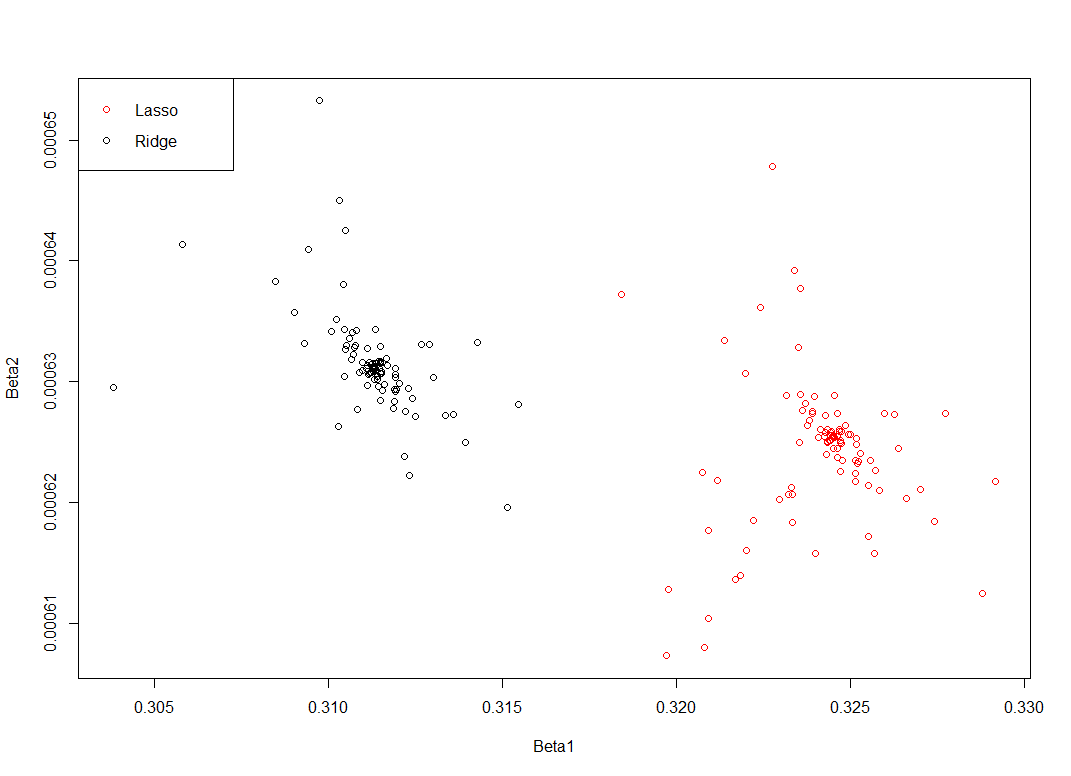
\includegraphics[width = 0.7\linewidth]{images/lasso-vs-ridge-instability.png}
	\label{fig:lasso-and-ridge-instability}
\end{figure}

\subsection{Elastic Net Regression}
Elastic net regression serves as a combination between ridge and lasso regression. It can handle  multicollinearity as well as perform variable selection. The coefficients for elastic net regression can be determined by 
\begin{equation}
	\hat{\beta}^{\text{ENet}}=\argmin{\beta}\left\{ \sum\limits_{i = 1}^n \left( y_i - \beta_0 - \sum\limits_{i = 1}^p \beta_j x_{ij} \right) + \lambda_2\sum\limits_{j = 1}^p \beta_j^2 + \lambda_1\sum\limits_{j = 1}^p \vert \beta_j \vert \right\}
\end{equation}
where $\lambda_1$ and $\lambda_2$ are both tuning parameters to be determined later.

An important limitation to note is that elastic net performs best when it close to either ridge or lasso regression, meaning that either $\lambda_1 >> \lambda_2$ or vice versa \cite{zou2005regularization}. Additionally, because elastic net requires two tuning parameters, this makes it much more difficult to determine the best combination of tuning parameters to minimize error in the regression. However, this problem has been largely solved through by the LARS-EN algorithm developed by Zou et. al. which efficiently solves for the tuning parameters.
% I will add more here later

\subsection{Adaptive Lasso Regression}
Normally in lasso regression, each predictor is weighted the same in the penalty function. Adaptive lasso regression is different in that a weight, $\hat{w}_j$ is multiplied to the penalty function. The coefficients for adaptive lasso regression as designed by Zou et. al. \cite{zou2006adaptive} can be defined by
\begin{equation}
	\hat{\beta}^{\text{adaptive}}=\argmin{\beta}\left\{ \sum\limits_{i = 1}^n \left( y_i - \beta_0 - \sum\limits_{i = 1}^p \beta_j x_{ij} \right) + \lambda\sum\limits_{j = 1}^p \hat{w}_j\vert \beta_j \vert \right\}
\end{equation}
where $\lambda$ is a tuning parameter to be determined later and $\hat{w}_j$ is defined as $\frac{1}{\vert\hat{\beta}\vert^{\gamma}}$ with $\gamma$ being a chosen parameter greater than 0.

Because of the weight that is implemented in adaptive lasso regression, zero-coefficients have a weight that is inflated up to infinity, and thus are punished much more harshly than large coefficients whose weight is much smaller in comparison. This is a similar rationale to SCAD and helps to reduce some of the bias from lasso regression. Bridge regression is the general form of lasso regression from which adaptive lasso originates from. When $\gamma < 1$, bridge regression as shown in Equation \ref{adap_lasso} is not continuous, which results in model prediction instability. However, adaptive lasso regression is completely continuous and thus has much more consistent coefficients when fitted.
% I will add more here in the future

\begin{equation}
	\hat{\beta}^{\text{lasso}}=\argmin{\beta}\left\{ \sum\limits_{i = 1}^n \left( y_i - \beta_0 - \sum\limits_{i = 1}^p \beta_j x_{ij} \right) + \lambda\sum\limits_{j = 1}^p \vert \beta_j \vert ^\gamma \right\}
	\label{adap_lasso}
\end{equation}


\subsection{Smoothly Clipped Absolute Deviation Regression}
One major flaw of the lasso method is that the penalty punishes large coefficients, even if those coefficients should be large. One way to modify the lasso method is to use the \textit{smoothly clipped absolute deviation} (SCAD) penalty \cite{fan2001variable}. The goal of this method is to punish large coefficients less severely, which can help mitigate some of the bias introduced by the lasso method.
\begin{equation}
	\hat{\beta}^{\text{SCAD}}=\argmin{\beta}\left\{ \sum\limits_{i = 1}^n \left( y_i - \beta_0 - \sum\limits_{i = 1}^p \beta_j x_{ij} \right) + \lambda\sum\limits_{j = 1}^p J_a(\beta_j, \lambda) \right\}
\end{equation}
Here, $J_a(\beta, \lambda)$ is a penalty function that satisfies
\begin{equation}
	\frac{dJ_a(\beta, \lambda)}{d\beta} = \lambda\cdot\sign(\beta)\left[ I(\vert \beta \vert<\lambda) + \frac{(a\lambda - \vert \beta\vert)_+}{(a - 1)\lambda}I(\vert \beta \vert > \lambda) \right]
\end{equation}
where $\lambda \geq 0$ and $a\geq 2$ are tuning parameters. An equivalent way to write this is
\begin{equation}
	\frac{dJ_a(\beta, \lambda)}{d\beta}\left\{\begin{array}{ll}
		\lambda,&\vert \beta \vert\leq \lambda\\
		\frac{a\lambda - \vert \beta \vert}{a - 1},&\lambda < \vert \beta \vert < a\lambda\\
		0,&\alpha\lambda < \vert \beta \vert
	\end{array}\right.
\end{equation}
This penalty function does not punish coefficients with large magnitude as heavily as the lasso method. In fact, if the magnitude of a coefficient is larger than $a\lambda$, then the penalty becomes constant. See Figure \ref{fig:penalty} for a plot of the SCAD penalty as a function of the coefficient value.

Integrating with respect to $\beta$ \cite{breheny2016lasso}, we see that
\begin{equation}
	J_a(\beta, \lambda) = \left\{\begin{array}{ll}
		\lambda \vert \beta \vert,&\vert \beta \vert \leq \lambda\\
		\frac{2a\lambda\vert\beta\vert - \beta^2-\lambda^2}{2(a - 1)},&\lambda < \vert \beta \vert < a\lambda\\
		\frac{\lambda^2(a + 1)}{2},&a\lambda < \vert \beta \vert
	\end{array}\right.
\end{equation}

\subsection{Minimax Concave Penalty Regression}
The minimax concave penalty (MCP) method is very similar to smoothly clipped absolute deviation \cite{zhang2010nearly, breheny2016lasso}. Both methods are used to avoid the high bias caused by the lasso method. MCP uses a penalty function that satisfies
\begin{equation}
	\frac{dJ_a(\beta, \lambda)}{d\beta} = \left\{\begin{array}{ll}
		\sign(\beta)\left(\lambda - \frac{\vert \beta \vert}{a}\right),& \vert \beta \vert \leq a\lambda\\
		0,&a\lambda < \vert \beta \vert
	\end{array}\right.
\end{equation}
where $\lambda\geq 0$ and $a> 0$ are tuning parameters. Integrating \cite{breheny2016lasso}, we see that
\begin{equation}
	J_a(\beta, \lambda) = \left\{\begin{array}{ll}
		\lambda \vert \beta \vert - \frac{\beta^2}{2a},&\vert \beta \vert \leq a\lambda\\
		\frac{1}{2}a\lambda^2,&a\lambda < \vert \beta \vert
	\end{array}\right.
\end{equation}

Figure \ref{fig:lasso-scad-mcp} below shows the penalty functions (and their derivatives) for LASSO, SCAD, and MCP as a function of a coefficient value $\beta$. We see that LASSO applies a much stronger penalty to large coefficients than SCAD or MCP. Also, note that SCAD starts with a derivative equal to that of the lasso for small values of $\beta$; on the other hand, the derivative of the penalty function for MCP starts decreasing immediately.

\begin{figure}[!h]
	\caption{Penalty functions for LASSO, SCAD, and MCP, as well as their derivatives. These plots use $\lambda = 2$ and $a = 3$.}
	\label{fig:lasso-scad-mcp}
	\centering
	\begin{subfigure}[b]{0.4\textwidth}
		\caption{Penalty functions for LASSO, SCAD, and MCP}
		\label{fig:penalty}
		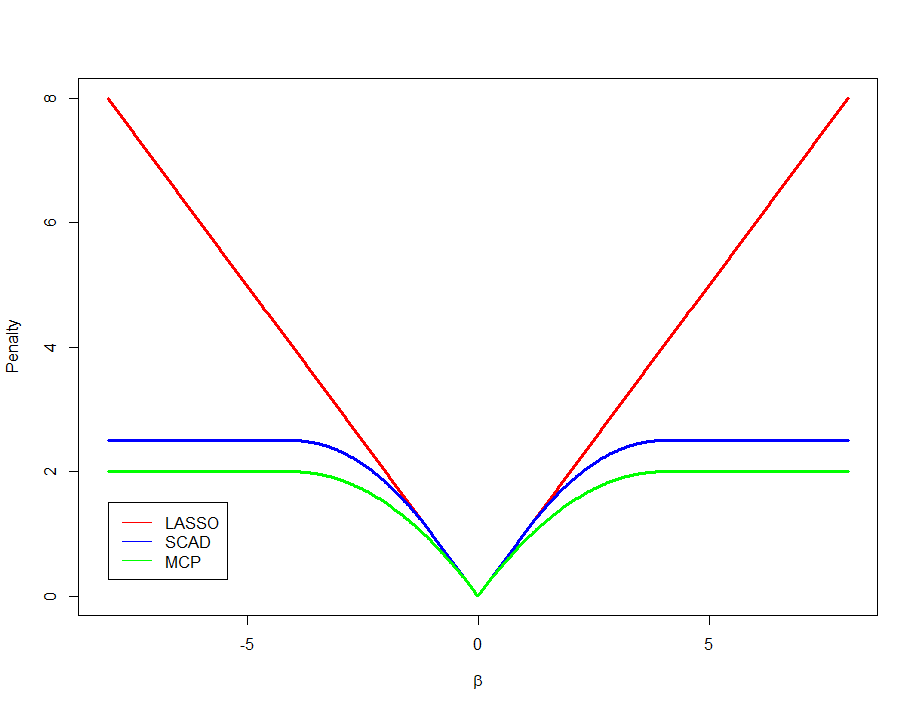
\includegraphics[width=\textwidth]{images/penalty.png}
	\end{subfigure}
	\hspace{30pt}
	\begin{subfigure}[b]{0.4\textwidth}
		\caption{Derivatives of the penalty functions for LASSO, SCAD, and MCP}
		\label{fig:derivative}
		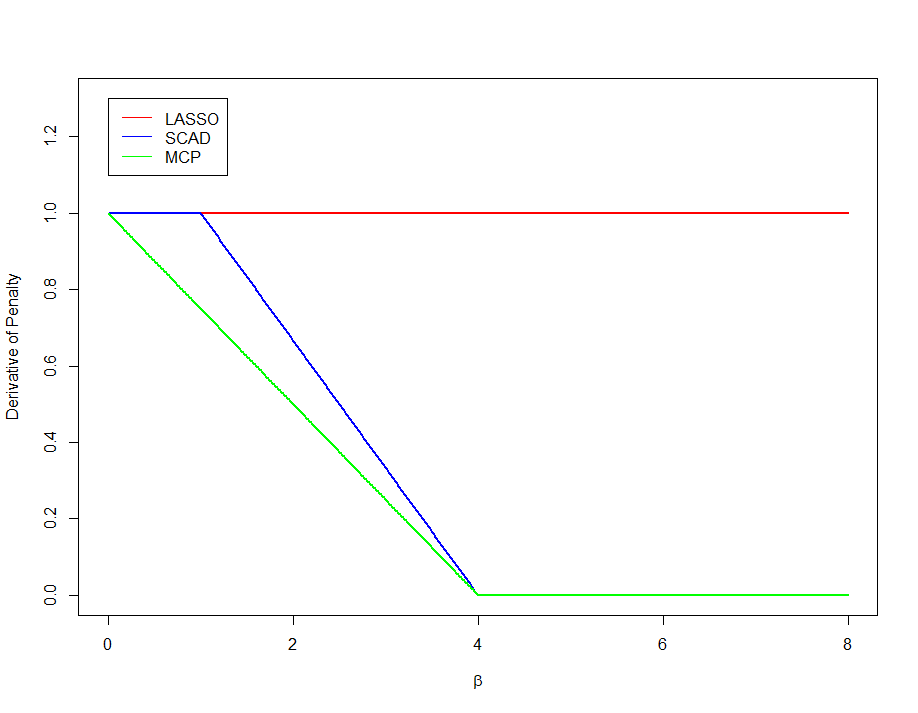
\includegraphics[width=\textwidth]{images/derivative.png}
	\end{subfigure}
\end{figure}

Now, consider the case where $p=1$ (there is only one predictor). Figure \ref{fig:prediction} shows the solutions given when using LASSO, SCAD, and MCP on such a model. The $x$-axis gives the actual coefficient for the single variable, and the $y$-axis represents the coefficient estimate produced using each of the algorithms. We used the particular values $\lambda = 2$ and $a = 3$. The gray line is the identity function, which also equals the solution obtained using ordinary least squares.

We see that all three methods set the predicted value to zero when the actual coefficient is small. Also, note that the LASSO method is always off from the identity function when the coefficient is large. On the other hand, SCAD and MCP merge with the identity function when the coefficient is sufficiently large. This shows that both SCAD and MCP can avoid the high bias that LASSO introduces.

\begin{figure}[!h]
	\centering
	\caption{Solutions for LASSO, SCAD, and MCP for a single predictor when $\lambda=2$, and $a = 3$.}
	\label{fig:prediction}
	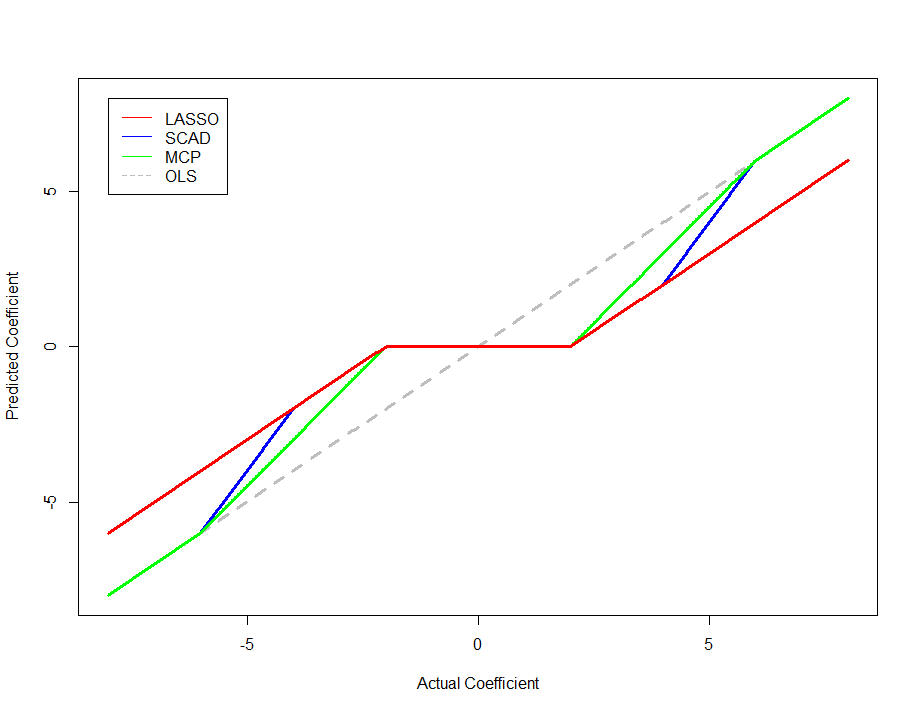
\includegraphics[width = 0.4\textwidth]{images/prediction.png}
\end{figure}

\newpage
\bibliographystyle{plain}
\bibliography{references}
\end{document}
